\chapter*{Representing a graph: graph learning techniques and dictionary representation}
In the previous section we presented the main reason why signal processing field expressed the necessity of having new different structures in order to better represent the amount of information we can collect from a phenomena: what we did not focused on yet, is the fact that these amount of data are usually largely redundant, since they are a densely sampled version of the signal and they may represent multiple correlated versions of the same physical event. So normally the significative information regarding the underlying processes is largely reducible in dimensionality with respect of the collected dataset. \cite{Tosic2011} Thus, we can obtain the data representations starting from the idea that our observations can be described by a sparse subset of elementary signals - so called \textit{atoms} - taken from an \textit{overcomplete dictionary}. When the dictionary forms a basis, then every signal can be univocally represented through the linear combination of the dictionary atoms, moreover the overcompleteness property \cri{definisci i significati delle n. Sei sicura che stai avendo a che fare con dizionari overcomplete? Si si } implies that atoms are linearly dependent. \cite{Tosic2011} \cite{Rubinstein2010}

With these premises, we consider a dictionary $\textbf{D} = [\textbf{d}_1, \textbf{d}_2, \dots, \textbf{d}_L] \in \R^{N \times L}$, in which the columns represent the dictionary atoms and, for the overcompleteness, $L\geq N$. Through this entity, the signal representations can be done through two main paths, either the \textit{synthesis} path, or the \textit{analysis} path, and the two can significantly differ in the overcomplete case.

In the synthesis path, the signal $\textbf{x} \in \R^N$ is represented as a linear combination of the dictionary atoms:
\begin{equation}
\textbf{x} = \textbf{D}^T \gamma_s
\label{eq:synthesis}
\end{equation}
while in the analysis path it is represented through its inner product with the atoms:
\begin{equation}
\gamma_a = \textbf{D}^T \textbf{x}
\label{eq:analysis}
\end{equation}

The representation in \ref{eq:synthesis} has the consequence that, when the dictionary is overcomplete, the set of representations $\gamma_s$satisfying the equation is \textit{infinitely large}, allowing us to look for the most informative representation of the signal with respect of a certain cost function $\mathcal{C}(\gamma)$. In this way we arrive to a first general optimization problem in the form:
\begin{equation}
\gamma_s = \argmin_{\gamma} \text{  } \mathcal{C}(\gamma) \quad \text{Subject To  } \textbf{x} = \textbf{$D\gamma$}
\label{eq:costF}
\end{equation}
The way we choose the form of the cost function obviously influences the structure of our solution, to be specific, one of our goals is to achieve sparsity in the representation of the signal, such that the signal reconstruction is reduced in dimensionality as we are trying to achieve from the beginning. Problem in \ref{eq:costF} becomes what is commonly referred as \textit{sparse coding}, and there are different functions we can apply in order to obtain it: these functions have the characteristic of being tolerant to large coefficients and at the same time importantly penalize small non-zero ones. Among these functions, our choice fell on the $l$ norm, which is one of the simplest and most effective function of this type.

\section{Choosing the right dictionary}
 What we did not focused on yet is the choice of the proper Dictionary for out task. In the research there has been so far, different models of Dictionaries have been defined and used for the most different purposes, in the beginning the attention was mainly on traditional dictionaries, such as wavelet and Fourier dictionaries, which are simple to use and perform well for 1-dimensional signals. However, these structures were too simple to properly describe more complex and high-dimensional data, so the focus slowly moved to seeking solutions that better performed in this environment. Dictionaries emerged from this need were coming from two main sources:
 \begin{itemize}
 \item As an \textit{analytical model}, which allows to extract the dictionary straight form the data for a fast implicit implementation that does not require multiplication by the dictionary matrix;
 \item As a \textit{set of realizations} of the data, which offers an increased flexibility and adaptability to data structure;
\end{itemize}
The first model prefers speed over adaptability, since its success depends on the chosen underlying model, sometimes resulting in a over-simplistic solution for the proposed problem. From this, the necessity of also focusing on the second type of dictionary, also defined as \textit{trained dictionary}.\\
Machine learning techniques of the period between 1980's and 1990's allowed to approach this problem under the new assumption that the structure of a natural phenomena can be accurately extracted \textit{straight form the data} with better results than using a mathematical formulation. The most recent training methods focus on the $l^0$ and $l^1$ sparsity measures, which have a simpler formulation and at the same time can use the more recent sparsity coding techniques. \cite{Gorodnitsky1997} \cite{Pati1993}
Among these learning methods, particular relevance acquired the \textit{parametric training methods}, such as \textit{translation-invariant dictionaries}, \textit{multiscale dictionaries} or \textit{sparse dictionaries}. These implementations involve the reduction of parameters' number and the assumption of several desirable properties on the dictionary, in the end leading to an accelerate convergence, reduced density of the local minima and the convergence to a better solution. Moreover, the generalization of the learning process is improved thanks to the smaller number of parameters, as much as the reduction in number of examples needed. Finally, parametric dictionaries bring to a more efficient implementation, due to the fact that parametrization typically has a more compact representation and, not less important, a parametric dictionary may be designed to represent infinite or arbitrary-sized signals. \cite{Rubinstein2010} \cri{forse aggiungi parte sugli sparse dictionaries sempre presa dallo stesso paper. Poi: vedi se aggiungere un excursus storico sui dizionari ad apprendimento}.
\subsubsection{The sparse approximation}
The intention of sparse approximations to represent a certain signal $y$ of dimension $n$ as the linear combination of a small amount of signals selected from the source database which is the dictionary and in which the elements typically are unit norm functions called \textit{atoms} and can be denoted through $\phi_k \text{ with } k = 1,\dots, N$ and being $N$ the size of the dictionary. When a dictionary is overcomplete, then every signal can be represented with the aforementioned linear combination:
\begin{equation}
\textbf{y} = \textbf{$\phi$}\textbf{a} = \sum_{k=1}^{N}a_k\phi_k
\end{equation}
and the value that \textbf{a} can assume is not unique.\\
To achieve sparse and efficient representations, the requirement for finding the exact representation is in general relaxed: starting from the NP-hard problem which is the minimization of the $l^0$ norm of \textbf{a}, we can approach the issue through convex relaxation methods that solve a problem in the form:
\begin{equation}
\min_\textbf{a} \text{ } (|| \textbf{y} - \textbf{$\phi$a} ||_2^2 + \textbf{$\lambda$}||\textbf{a}||_1)
\end{equation}
in which the relaxation allowed to replace the nonconvex $l^0$ norm in the original problem with a more meaningful $l^1$ norm. \cite{Tosic2011}

\section{The correspondence between the dictionary and the graph signal}
In \ref{sec:graph laplacian} we introduced the Laplacian operator as $L = D - W$, here we focus on a modified version of this operator, that is the \textit{normalized Laplacian} $\mathcal{L} = D^{-\frac{1}{2}}LD^{-\frac{1}{2}}$, also a real symmetric and positive semidefinite matrix, with a complete set of orthonormal eigenvectors $\textbf{$\chi$} = [\chi_0,\chi_1,\dots,\chi_{N-1}]$ and associated non negative eigenvalues $\sigma(\mathcal{L}) := \{ 0 = \lambda_0,\lambda_1,\dots,\lambda{N-1} \leq 2 \}$ (where the upper bound 2 comes from the normalization).
The normalized Laplacian eigenvectors are Fourier basis, this bringing any function $y$ defined on the vertices of the graph to be represented in his Fourier transform version $\hat{y}$ at frequency $\lambda_l$ as:
\begin{equation}
\hat{y}(\lambda_l) = \langle y, \chi_l \rangle = \sum_{n=1}^{N} y(n)\chi_l^{*}(n)
\end{equation}
and its relative inverse transform to be:
\begin{equation}
y(n) = \sum_{l=0}^{N-1} \hat{y}(\lambda_l)\chi_l(n), \quad \forall n \in \mathcal{V}
\end{equation}
This transform plays a major role not only in the harmonic analysis, but also in defining the signal translation onto a graph. It is worth to notice here that in the classical signal processing field the translation operator is defined through the change of variable $(T_n f)(t) := f(t-n)$, but when it comes to graph signal processing, this concept looses meaning since there is no significate to $f(\circ - n)$ in the graph environment. However, from transform theory we can recall that the classical translation operator $T_n$ can also be seen as a convolution with a Kronecker delta $\delta$ centered in $n$\cite{Shuman2013} \cite{Thanou2014}:
\begin{equation}
T_n g = \sqrt{N}(g * \delta_n) = \sqrt{N}\sum_{l=0}^{N-1}\hat{g}(\lambda_l)\chi_l^{*}(n)\chi_l
\label{eq:translation}
\end{equation}

this leading to think about \ref{eq:translation} as an operator acting on the kernel $g(\cdot)$ directly defined in the spectral domain and from which we can obtain the effective translation to kernel $n$ through inverse graph Fourier transform. Moreover the term $\sqrt{N}$ in the \autoref{eq:translation} is a guarantee for the translation operator to preserve the mean of the signal, while the $g(\cdot)$ kernel smoothness is a measure to control the localization of $T_n g$ centered at vertex $n$ (meaning that the magnitude ($T_n g$)(i) of the translated kernel at vertex $i$ decays with the increasing distance from the center of the kernel). We can thus compose our atoms $T_n g$ as smooth entities, coming from the assumption that the kernel function in \ref{eq:translation} is a smooth polynomial function of degree K:
\begin{equation}
\hat{g}(\lambda_l) = \sum_{k=0}^{K} \alpha_k\lambda_l^k, \quad l = 0,\dots,N-1
\end{equation}
From this fact, we can so obtain a global expression for a translation operator as:
\begin{align}
T_n g & = \sqrt{N}(g * \delta_n) = \sqrt{N}\sum_{l=0}^{N-1}\sum_{k=0}^{K}\alpha_k\lambda_l^k\chi_l^*(n)\chi_l \\
&= \sqrt{N}\sum_{k=0}^{K}\alpha_k\sum_{l=0}^{N-1}\lambda_l^k\chi_l^*(n)\chi_l = \sqrt{N}\sum_{k=0}^{K}\alpha_k (\mathcal{L}^k)_n
\end{align}
where $(\mathcal{L})_n$ represents the $n^{th}$ column of the $k^{th}$ power of the Laplacian matrix $\mathcal{L}^k$. The final concatenation of $N$ such columns brings us to generate a set of $N$ atoms, corresponding to the columns of
\begin{equation}
Tg = \sqrt{N}\hat{g}(\mathcal{L}) = \sqrt{N}\chi \hat{g}(\Lambda)\chi^T = \sqrt{N}\sum_{k=0}^{K}\alpha_k\mathcal{L}^k
\label{eq:tg}
\end{equation}
Where the quantity $\Lambda$ corresponds to the diagonal matrix of the eigenvalues in such a way that the following relation holds: $\mathcal{L} = \rchi \Lambda \rchi^T$ \cite{Dong2016}. This brief section has the intrinsic meaning that if the kernel $g(\cdot)$ is a polynomial of degree $K$, then the translation operator is $0$ in all the vertices $i$ that are more than $K$ hops far away from the center vertex $n$, which means that the vertex domain support of the translated vertex is contained in a sphere of radius $K$ and center in $n$ and its magnitude decades with the increasing distance from $n$ to $i$.
In \autoref{fig:minnesota} there is an example of an atom translation in three different ways.

\begin{figure}
\centering
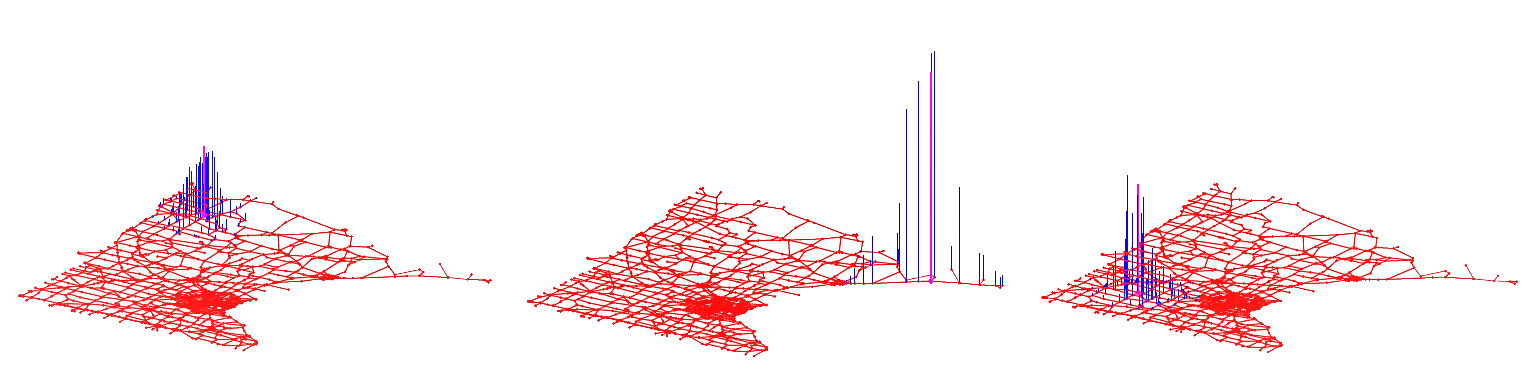
\includegraphics[width = 1\textwidth]{MinnesotaTranslation.png}
\caption{Example of graph signal translation: translation for $T_{200}g$ (a), $T_{1000}g$ (b) and $T_{2000}g$ (c)}
\label{fig:minnesota}
\end{figure}
